\documentclass[11pt, answers]{exam}
\usepackage[margin=1in]{geometry}
\usepackage{amsfonts, amsmath, amssymb, amsthm}
\usepackage{mathtools}
\usepackage{enumerate}
\usepackage{listings}
\usepackage{cancel}
\usepackage{hyperref}
\usepackage[boxed]{algorithm}
\usepackage[noend]{algpseudocode}
\usepackage{tikz}
\usepackage{float}
\usepackage{MnSymbol}

%
% Basic Document Settings
%

\topmargin=-0.45in
\evensidemargin=0in
\oddsidemargin=0in
\textwidth=6.5in
\textheight=9.0in
\headsep=0.25in

\linespread{1.1}

\pagestyle{headandfoot}
\lhead{\hmwkClass\ : \hmwkType\ \#\hmwkNumber\ (Due \hmwkDue)}
\cfoot{\thepage}
% \renewcommand\headrulewidth{0.4pt}
% \renewcommand\footrulewidth{0.4pt}

\setlength\parindent{0pt}

%
% Create Problem Sections
%
\qformat{\hfill}

\newcommand{\hmwkType}{Electronic}
\newcommand{\hmwkNumber}{6}
\newcommand{\hmwkClass}{VE 492}
\newcommand{\hmwkDue}{July 1st, 2020 at 11:59pm}


%
% Title Page
%

\title{Homework \hmwkNumber\ \hmwkType}
\date{\hmwkDue}

%
% Various Helper Commands
%

% space of real numbers \R
\newcommand{\R}{\mathbb{R}}

% expected value \EX
\DeclareMathOperator{\EX}{\mathbb{E}}

% For partial derivatives \pderiv{}{}
\newcommand{\pderiv}[2]{\frac{\partial}{\partial #1} (#2)}

% argmax \argmax
\DeclareMathOperator*{\argmax}{arg\,max}

% sign \sign
\DeclareMathOperator{\sign}{sign}

% norm \norm{}
\DeclarePairedDelimiter{\norm}{\lVert}{\rVert}

% Keys
\newcommand{\key}[1]{\fbox{{\sc #1}}}
\newcommand{\ctrl}{\key{ctrl}--}
\newcommand{\shift}{\key{shift}--}
\newcommand{\run}{\key{run} \ }
\newcommand{\runkey}[1]{\run \key{#1}}
\newcommand{\extend}{\key{extend} \ }
\newcommand{\kkey}[1]{\key{k$_{#1}$}}

\begin{document}
\maketitle

\section{Probability}
    \begin{enumerate}[a]
    \item
    \begin{enumerate}[i]
    \item
    Not possible
    \item
    $\dfrac{P(A)P(B|A)P(C|A,B)}{\sum_bP(A)P(B|A)P(C|A,B)}$
    \item
    $\sum_aP(A|B)P(C|A)$
    \item
    Not possible
    \end{enumerate}
    \item
    \begin{enumerate}[i]
    \item
    $A\upmodels C$, $A\upmodels B$
    \item
    $B\upmodels C\vert A$
    \item
    No independence assumptions needed.
   	\item
   	No independence assumptions needed.
    \end{enumerate}
    \item
    (i) (ii) (iii)
		\begin{figure}[h]
		\centering
		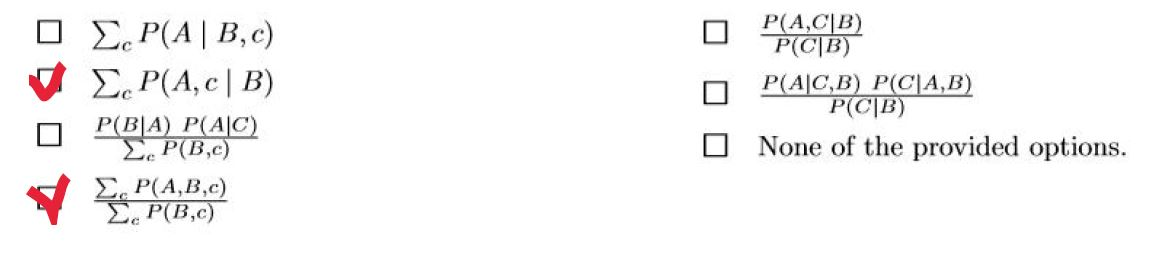
\includegraphics[scale=0.5]{1.jpg}
		\end{figure}
		
		\begin{figure}[h]
		\centering
		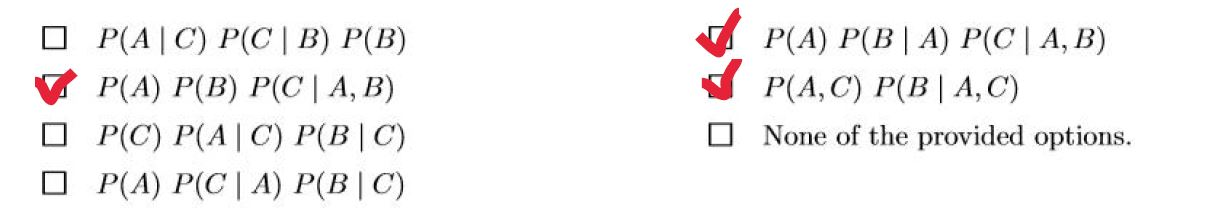
\includegraphics[scale=0.5]{2.jpg}
		\end{figure}
		
		\begin{figure}[h]
		\centering
		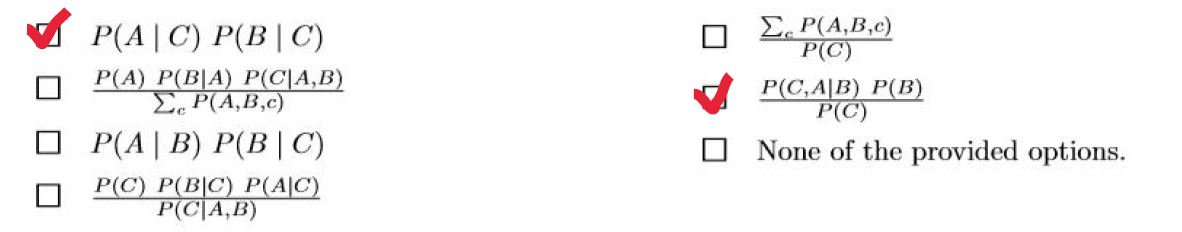
\includegraphics[scale=0.5]{3.jpg}
		\end{figure}
    \end{enumerate}



\end{document}
